% Options for packages loaded elsewhere
\PassOptionsToPackage{unicode}{hyperref}
\PassOptionsToPackage{hyphens}{url}
\documentclass[
  11pt,
]{article}
\usepackage{xcolor}
\usepackage[margin=1in]{geometry}
\usepackage{amsmath,amssymb}
\setcounter{secnumdepth}{5}
\usepackage{iftex}
\ifPDFTeX
  \usepackage[T1]{fontenc}
  \usepackage[utf8]{inputenc}
  \usepackage{textcomp} % provide euro and other symbols
\else % if luatex or xetex
  \usepackage{unicode-math} % this also loads fontspec
  \defaultfontfeatures{Scale=MatchLowercase}
  \defaultfontfeatures[\rmfamily]{Ligatures=TeX,Scale=1}
\fi
\usepackage{lmodern}
\ifPDFTeX\else
  % xetex/luatex font selection
\fi
% Use upquote if available, for straight quotes in verbatim environments
\IfFileExists{upquote.sty}{\usepackage{upquote}}{}
\IfFileExists{microtype.sty}{% use microtype if available
  \usepackage[]{microtype}
  \UseMicrotypeSet[protrusion]{basicmath} % disable protrusion for tt fonts
}{}
\makeatletter
\@ifundefined{KOMAClassName}{% if non-KOMA class
  \IfFileExists{parskip.sty}{%
    \usepackage{parskip}
  }{% else
    \setlength{\parindent}{0pt}
    \setlength{\parskip}{6pt plus 2pt minus 1pt}}
}{% if KOMA class
  \KOMAoptions{parskip=half}}
\makeatother
\usepackage{color}
\usepackage{fancyvrb}
\newcommand{\VerbBar}{|}
\newcommand{\VERB}{\Verb[commandchars=\\\{\}]}
\DefineVerbatimEnvironment{Highlighting}{Verbatim}{commandchars=\\\{\}}
% Add ',fontsize=\small' for more characters per line
\usepackage{framed}
\definecolor{shadecolor}{RGB}{248,248,248}
\newenvironment{Shaded}{\begin{snugshade}}{\end{snugshade}}
\newcommand{\AlertTok}[1]{\textcolor[rgb]{0.94,0.16,0.16}{#1}}
\newcommand{\AnnotationTok}[1]{\textcolor[rgb]{0.56,0.35,0.01}{\textbf{\textit{#1}}}}
\newcommand{\AttributeTok}[1]{\textcolor[rgb]{0.13,0.29,0.53}{#1}}
\newcommand{\BaseNTok}[1]{\textcolor[rgb]{0.00,0.00,0.81}{#1}}
\newcommand{\BuiltInTok}[1]{#1}
\newcommand{\CharTok}[1]{\textcolor[rgb]{0.31,0.60,0.02}{#1}}
\newcommand{\CommentTok}[1]{\textcolor[rgb]{0.56,0.35,0.01}{\textit{#1}}}
\newcommand{\CommentVarTok}[1]{\textcolor[rgb]{0.56,0.35,0.01}{\textbf{\textit{#1}}}}
\newcommand{\ConstantTok}[1]{\textcolor[rgb]{0.56,0.35,0.01}{#1}}
\newcommand{\ControlFlowTok}[1]{\textcolor[rgb]{0.13,0.29,0.53}{\textbf{#1}}}
\newcommand{\DataTypeTok}[1]{\textcolor[rgb]{0.13,0.29,0.53}{#1}}
\newcommand{\DecValTok}[1]{\textcolor[rgb]{0.00,0.00,0.81}{#1}}
\newcommand{\DocumentationTok}[1]{\textcolor[rgb]{0.56,0.35,0.01}{\textbf{\textit{#1}}}}
\newcommand{\ErrorTok}[1]{\textcolor[rgb]{0.64,0.00,0.00}{\textbf{#1}}}
\newcommand{\ExtensionTok}[1]{#1}
\newcommand{\FloatTok}[1]{\textcolor[rgb]{0.00,0.00,0.81}{#1}}
\newcommand{\FunctionTok}[1]{\textcolor[rgb]{0.13,0.29,0.53}{\textbf{#1}}}
\newcommand{\ImportTok}[1]{#1}
\newcommand{\InformationTok}[1]{\textcolor[rgb]{0.56,0.35,0.01}{\textbf{\textit{#1}}}}
\newcommand{\KeywordTok}[1]{\textcolor[rgb]{0.13,0.29,0.53}{\textbf{#1}}}
\newcommand{\NormalTok}[1]{#1}
\newcommand{\OperatorTok}[1]{\textcolor[rgb]{0.81,0.36,0.00}{\textbf{#1}}}
\newcommand{\OtherTok}[1]{\textcolor[rgb]{0.56,0.35,0.01}{#1}}
\newcommand{\PreprocessorTok}[1]{\textcolor[rgb]{0.56,0.35,0.01}{\textit{#1}}}
\newcommand{\RegionMarkerTok}[1]{#1}
\newcommand{\SpecialCharTok}[1]{\textcolor[rgb]{0.81,0.36,0.00}{\textbf{#1}}}
\newcommand{\SpecialStringTok}[1]{\textcolor[rgb]{0.31,0.60,0.02}{#1}}
\newcommand{\StringTok}[1]{\textcolor[rgb]{0.31,0.60,0.02}{#1}}
\newcommand{\VariableTok}[1]{\textcolor[rgb]{0.00,0.00,0.00}{#1}}
\newcommand{\VerbatimStringTok}[1]{\textcolor[rgb]{0.31,0.60,0.02}{#1}}
\newcommand{\WarningTok}[1]{\textcolor[rgb]{0.56,0.35,0.01}{\textbf{\textit{#1}}}}
\usepackage{longtable,booktabs,array}
\newcounter{none} % for unnumbered tables
\usepackage{calc} % for calculating minipage widths
% Correct order of tables after \paragraph or \subparagraph
\usepackage{etoolbox}
\makeatletter
\patchcmd\longtable{\par}{\if@noskipsec\mbox{}\fi\par}{}{}
\makeatother
% Allow footnotes in longtable head/foot
\IfFileExists{footnotehyper.sty}{\usepackage{footnotehyper}}{\usepackage{footnote}}
\makesavenoteenv{longtable}
\usepackage{graphicx}
\makeatletter
\newsavebox\pandoc@box
\newcommand*\pandocbounded[1]{% scales image to fit in text height/width
  \sbox\pandoc@box{#1}%
  \Gscale@div\@tempa{\textheight}{\dimexpr\ht\pandoc@box+\dp\pandoc@box\relax}%
  \Gscale@div\@tempb{\linewidth}{\wd\pandoc@box}%
  \ifdim\@tempb\p@<\@tempa\p@\let\@tempa\@tempb\fi% select the smaller of both
  \ifdim\@tempa\p@<\p@\scalebox{\@tempa}{\usebox\pandoc@box}%
  \else\usebox{\pandoc@box}%
  \fi%
}
% Set default figure placement to htbp
\def\fps@figure{htbp}
\makeatother
\setlength{\emergencystretch}{3em} % prevent overfull lines
\providecommand{\tightlist}{%
  \setlength{\itemsep}{0pt}\setlength{\parskip}{0pt}}
\usepackage{amsmath}
% Shared LaTeX preamble for all Data Mining / ISLR chapter documents.
% Provides \makecoverpage{<assignment title>} — a standalone title page
% with fixed student identity, so every chapter/lab looks uniform.

\usepackage{graphicx}

\newcommand{\makecoverpage}[1]{%
\begin{titlepage}
\centering
\vspace*{2cm}

{\Large \textbf{Adventist University of Central Africa}}\\[0.4cm]
{\large Master's in Big Data Analytics}\\[2cm]

{\Huge \textbf{#1}}\\[0.5cm]
{\large \textit{Introduction to Statistical Learning with Applications in R}}\\[3cm]

\begin{tabular}{rl}
\textbf{Programme:} & MSc Big Data Analytics \\
\textbf{Course Title:} & Data Mining \\
\textbf{Course Code:} & MSDA 9124 \\
\textbf{Lecturer:} & Dr. Pacifique Nizeyimana \\
\textbf{Student Name:} & Wayne Rubangisa \\
\textbf{Student ID:} & 101220 \\
\end{tabular}

\vfill

{\large September 2026}

\end{titlepage}
}

\usepackage{bookmark}
\IfFileExists{xurl.sty}{\usepackage{xurl}}{} % add URL line breaks if available
\urlstyle{same}
\hypersetup{
  hidelinks,
  pdfcreator={LaTeX via pandoc}}

\author{}
\date{\vspace{-2.5em}}

\begin{document}

\makecoverpage{Chapter 12 --- Unsupervised Learning \\ Lab}

\begin{Shaded}
\begin{Highlighting}[]
\FunctionTok{library}\NormalTok{(ISLR2)}
\end{Highlighting}
\end{Shaded}

\section{Introduction}\label{introduction}

Supervised learning has a response variable that tells us what we are
trying to predict. Unsupervised learning starts without that response.
Instead, it looks for useful structure in the predictors themselves.

This lab develops the main tools from Chapter 12 of \emph{An
Introduction to Statistical Learning}:

\begin{enumerate}
\def\labelenumi{\arabic{enumi}.}
\tightlist
\item
  principal component analysis (PCA), which replaces many correlated
  predictors with a smaller number of directions that explain their
  shared variation;
\item
  hierarchical clustering, which builds a tree of increasingly large
  clusters; and
\item
  \(K\)-means clustering, which directly searches for a chosen number of
  compact groups.
\end{enumerate}

The methods answer related but different questions. PCA is primarily a
continuous dimension-reduction method. Clustering is primarily a
grouping method. Neither method automatically discovers the one true
answer: the analyst must choose scales, distances, tuning values, and
interpretations carefully.

\section{Principal Component
Analysis}\label{principal-component-analysis}

\subsection{Why dimension reduction is
useful}\label{why-dimension-reduction-is-useful}

Suppose a dataset contains \(p\) quantitative variables. Plotting or
modelling all \(p\) variables can be difficult, especially when several
variables measure similar underlying phenomena. PCA constructs new
variables called principal components. Each component is a linear
combination of the original variables:

\[
Z_m = \phi_{1m}X_1 + \phi_{2m}X_2 + \cdots + \phi_{pm}X_p.
\]

The loading vector \(\phi_m=(\phi_{1m},\ldots,\phi_{pm})\) determines
the direction of the component. PCA chooses the first direction to
maximise the variance of the projected observations, subject to
\(\|\phi_1\|=1\):

\[
\phi_1 = \arg\max_{\|\phi\|=1}
\operatorname{Var}(X\phi).
\]

The second component is the direction with the largest remaining
variance, subject to being orthogonal to the first, and so on. The
components are uncorrelated by construction and are ordered from
greatest to least variance.

\subsection{\texorpdfstring{PCA with the \texttt{USArrests}
data}{PCA with the USArrests data}}\label{pca-with-the-usarrests-data}

\texttt{USArrests} contains four crime-related measurements for the 50
US states. The variables are measured on different scales, so the
analysis should standardize them first. Otherwise, a variable with
larger numerical units would influence the components more heavily even
if it were not more informative.

\begin{Shaded}
\begin{Highlighting}[]
\FunctionTok{data}\NormalTok{(USArrests)}
\FunctionTok{summary}\NormalTok{(USArrests)}
\end{Highlighting}
\end{Shaded}

\begin{verbatim}
##      Murder          Assault         UrbanPop          Rape      
##  Min.   : 0.800   Min.   : 45.0   Min.   :32.00   Min.   : 7.30  
##  1st Qu.: 4.075   1st Qu.:109.0   1st Qu.:54.50   1st Qu.:15.07  
##  Median : 7.250   Median :159.0   Median :66.00   Median :20.10  
##  Mean   : 7.788   Mean   :170.8   Mean   :65.54   Mean   :21.23  
##  3rd Qu.:11.250   3rd Qu.:249.0   3rd Qu.:77.75   3rd Qu.:26.18  
##  Max.   :17.400   Max.   :337.0   Max.   :91.00   Max.   :46.00
\end{verbatim}

\begin{Shaded}
\begin{Highlighting}[]
\NormalTok{USArrests\_scaled }\OtherTok{\textless{}{-}} \FunctionTok{scale}\NormalTok{(USArrests)}
\FunctionTok{apply}\NormalTok{(USArrests\_scaled, }\DecValTok{2}\NormalTok{, mean)}
\end{Highlighting}
\end{Shaded}

\begin{verbatim}
##        Murder       Assault      UrbanPop          Rape 
##  1.543210e-16  1.143530e-16 -3.996803e-16  8.526513e-16
\end{verbatim}

\begin{Shaded}
\begin{Highlighting}[]
\FunctionTok{apply}\NormalTok{(USArrests\_scaled, }\DecValTok{2}\NormalTok{, sd)}
\end{Highlighting}
\end{Shaded}

\begin{verbatim}
##   Murder  Assault UrbanPop     Rape 
##        1        1        1        1
\end{verbatim}

The sample covariance matrix shows how the original variables move
together. PCA diagonalizes this covariance matrix: its eigenvectors give
the loading vectors, and its eigenvalues give the variances of the
corresponding components.

\begin{Shaded}
\begin{Highlighting}[]
\NormalTok{usarrests.pca }\OtherTok{\textless{}{-}} \FunctionTok{prcomp}\NormalTok{(USArrests, }\AttributeTok{scale. =} \ConstantTok{TRUE}\NormalTok{)}
\FunctionTok{summary}\NormalTok{(usarrests.pca)}
\end{Highlighting}
\end{Shaded}

\begin{verbatim}
## Importance of components:
##                           PC1    PC2     PC3     PC4
## Standard deviation     1.5749 0.9949 0.59713 0.41645
## Proportion of Variance 0.6201 0.2474 0.08914 0.04336
## Cumulative Proportion  0.6201 0.8675 0.95664 1.00000
\end{verbatim}

The standard deviations reported by \texttt{prcomp()} are the square
roots of the component variances. The proportion of variance explained
by component \(m\) is therefore

\[
\operatorname{PVE}_m =
\frac{d_m^2}{\sum_{j=1}^{p}d_j^2},
\]

where \(d_m\) is the reported standard deviation of component \(m\). The
cumulative PVE tells us how many components are needed to retain a
chosen amount of total variation.

\begin{Shaded}
\begin{Highlighting}[]
\NormalTok{usarrests\_pve }\OtherTok{\textless{}{-}} \FunctionTok{data.frame}\NormalTok{(}
  \AttributeTok{Component =} \FunctionTok{seq\_along}\NormalTok{(usarrests.pca}\SpecialCharTok{$}\NormalTok{sdev),}
  \AttributeTok{Standard\_deviation =}\NormalTok{ usarrests.pca}\SpecialCharTok{$}\NormalTok{sdev,}
  \AttributeTok{Proportion\_variance =}\NormalTok{ usarrests.pca}\SpecialCharTok{$}\NormalTok{sdev}\SpecialCharTok{\^{}}\DecValTok{2} \SpecialCharTok{/}
    \FunctionTok{sum}\NormalTok{(usarrests.pca}\SpecialCharTok{$}\NormalTok{sdev}\SpecialCharTok{\^{}}\DecValTok{2}\NormalTok{),}
  \AttributeTok{Cumulative\_variance =} \FunctionTok{cumsum}\NormalTok{(usarrests.pca}\SpecialCharTok{$}\NormalTok{sdev}\SpecialCharTok{\^{}}\DecValTok{2}\NormalTok{) }\SpecialCharTok{/}
    \FunctionTok{sum}\NormalTok{(usarrests.pca}\SpecialCharTok{$}\NormalTok{sdev}\SpecialCharTok{\^{}}\DecValTok{2}\NormalTok{)}
\NormalTok{)}
\NormalTok{usarrests\_pve}
\end{Highlighting}
\end{Shaded}

\begin{verbatim}
##   Component Standard_deviation Proportion_variance Cumulative_variance
## 1         1          1.5748783          0.62006039           0.6200604
## 2         2          0.9948694          0.24744129           0.8675017
## 3         3          0.5971291          0.08914080           0.9566425
## 4         4          0.4164494          0.04335752           1.0000000
\end{verbatim}

\begin{Shaded}
\begin{Highlighting}[]
\FunctionTok{plot}\NormalTok{(usarrests\_pve}\SpecialCharTok{$}\NormalTok{Component, usarrests\_pve}\SpecialCharTok{$}\NormalTok{Proportion\_variance,}
     \AttributeTok{type =} \StringTok{"b"}\NormalTok{, }\AttributeTok{pch =} \DecValTok{19}\NormalTok{,}
     \AttributeTok{xlab =} \StringTok{"Principal component"}\NormalTok{,}
     \AttributeTok{ylab =} \StringTok{"Proportion of variance explained"}\NormalTok{,}
     \AttributeTok{main =} \StringTok{"USArrests: scree plot"}\NormalTok{)}
\end{Highlighting}
\end{Shaded}

\begin{center}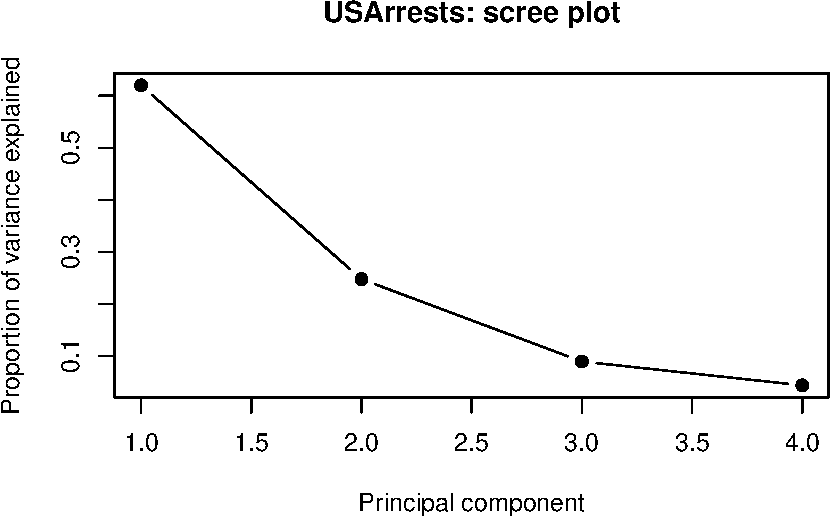
\includegraphics{ch12_lab_files/figure-latex/pca-usarrests-scree-1} \end{center}

The loadings show which original variables contribute to each direction.
A large absolute loading means that the variable is important for that
component; the sign is a direction convention, because multiplying an
entire component by \(-1\) gives the same underlying axis.

\begin{Shaded}
\begin{Highlighting}[]
\FunctionTok{round}\NormalTok{(usarrests.pca}\SpecialCharTok{$}\NormalTok{rotation, }\DecValTok{3}\NormalTok{)}
\end{Highlighting}
\end{Shaded}

\begin{verbatim}
##             PC1    PC2    PC3    PC4
## Murder   -0.536 -0.418  0.341  0.649
## Assault  -0.583 -0.188  0.268 -0.743
## UrbanPop -0.278  0.873  0.378  0.134
## Rape     -0.543  0.167 -0.818  0.089
\end{verbatim}

The first component often places violent and property crime measures in
a similar direction, while the second contrasts the variables that
behave differently. This interpretation should be made from the loading
pattern, not from the component name alone.

\subsection{Visualising observations in component
space}\label{visualising-observations-in-component-space}

\begin{Shaded}
\begin{Highlighting}[]
\FunctionTok{biplot}\NormalTok{(usarrests.pca, }\AttributeTok{scale =} \DecValTok{0}\NormalTok{, }\AttributeTok{cex =} \FloatTok{0.7}\NormalTok{,}
       \AttributeTok{main =} \StringTok{"USArrests represented in the first two PCs"}\NormalTok{)}
\end{Highlighting}
\end{Shaded}

\begin{center}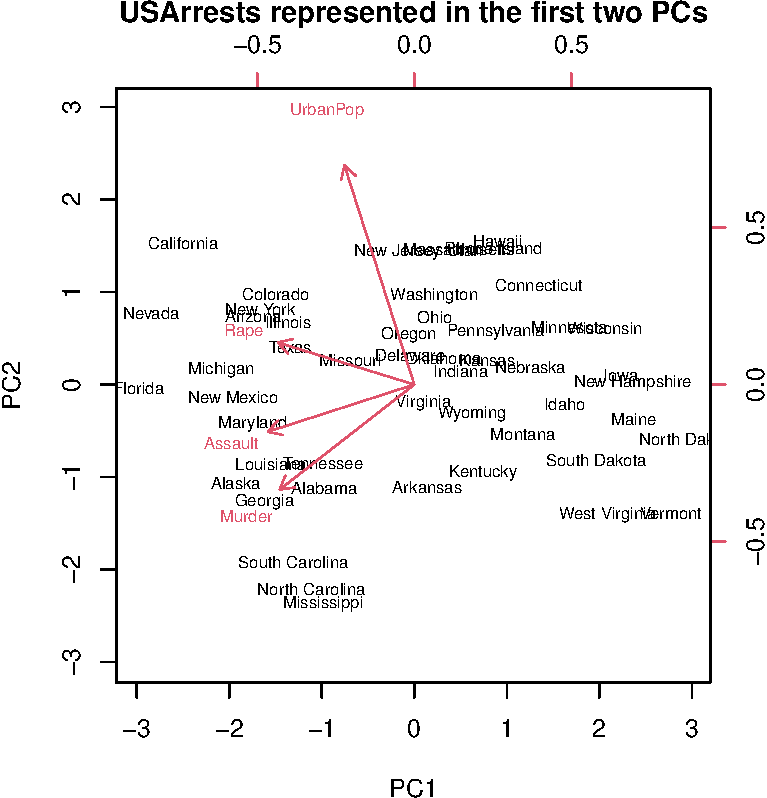
\includegraphics{ch12_lab_files/figure-latex/pca-usarrests-biplot-1} \end{center}

A biplot displays both observations and variable directions. States that
are near one another have similar standardized crime profiles. Variables
pointing in similar directions are positively associated; variables
pointing in opposite directions are negatively associated in the
displayed component plane.

\section{Hierarchical Clustering}\label{hierarchical-clustering}

\subsection{Distances and linkage}\label{distances-and-linkage}

Clustering begins with a measure of dissimilarity between observations.
With standardized quantitative variables, Euclidean distance between
observations \(i\) and \(j\) is

\[
 d(i,j) = \sqrt{\sum_{k=1}^{p}(x_{ik}-x_{jk})^2}.
\]

Hierarchical clustering initially treats every observation as its own
cluster. At each step it merges the two closest clusters and records the
fusion distance. The complete sequence of merges is represented by a
dendrogram.

Different linkage rules define cluster distance differently. For
clusters \(A\) and \(B\):

\[
D_{\mathrm{single}}(A,B) = \min_{i\in A,j\in B}d(i,j),
\]

\[
D_{\mathrm{complete}}(A,B) = \max_{i\in A,j\in B}d(i,j),
\]

and average linkage uses the mean of all cross-cluster distances. Single
linkage can join groups through chains of nearby observations, while
complete linkage tends to favour compact groups.

\subsection{\texorpdfstring{\texttt{USArrests}
dendrograms}{USArrests dendrograms}}\label{usarrests-dendrograms}

We use the standardized data so that the distance is not dominated by
the measurement units of a single variable.

\begin{Shaded}
\begin{Highlighting}[]
\NormalTok{distance.usarrests }\OtherTok{\textless{}{-}} \FunctionTok{dist}\NormalTok{(USArrests\_scaled)}

\NormalTok{hc.complete }\OtherTok{\textless{}{-}} \FunctionTok{hclust}\NormalTok{(distance.usarrests, }\AttributeTok{method =} \StringTok{"complete"}\NormalTok{)}
\NormalTok{hc.average }\OtherTok{\textless{}{-}} \FunctionTok{hclust}\NormalTok{(distance.usarrests, }\AttributeTok{method =} \StringTok{"average"}\NormalTok{)}
\NormalTok{hc.single }\OtherTok{\textless{}{-}} \FunctionTok{hclust}\NormalTok{(distance.usarrests, }\AttributeTok{method =} \StringTok{"single"}\NormalTok{)}
\end{Highlighting}
\end{Shaded}

\begin{Shaded}
\begin{Highlighting}[]
\FunctionTok{par}\NormalTok{(}\AttributeTok{mfrow =} \FunctionTok{c}\NormalTok{(}\DecValTok{3}\NormalTok{, }\DecValTok{1}\NormalTok{), }\AttributeTok{mar =} \FunctionTok{c}\NormalTok{(}\DecValTok{3}\NormalTok{, }\DecValTok{4}\NormalTok{, }\DecValTok{3}\NormalTok{, }\DecValTok{1}\NormalTok{))}
\FunctionTok{plot}\NormalTok{(hc.complete, }\AttributeTok{main =} \StringTok{"Complete linkage"}\NormalTok{, }\AttributeTok{xlab =} \StringTok{""}\NormalTok{, }\AttributeTok{sub =} \StringTok{""}\NormalTok{)}
\FunctionTok{plot}\NormalTok{(hc.average, }\AttributeTok{main =} \StringTok{"Average linkage"}\NormalTok{, }\AttributeTok{xlab =} \StringTok{""}\NormalTok{, }\AttributeTok{sub =} \StringTok{""}\NormalTok{)}
\FunctionTok{plot}\NormalTok{(hc.single, }\AttributeTok{main =} \StringTok{"Single linkage"}\NormalTok{, }\AttributeTok{xlab =} \StringTok{""}\NormalTok{, }\AttributeTok{sub =} \StringTok{""}\NormalTok{)}
\end{Highlighting}
\end{Shaded}

\begin{center}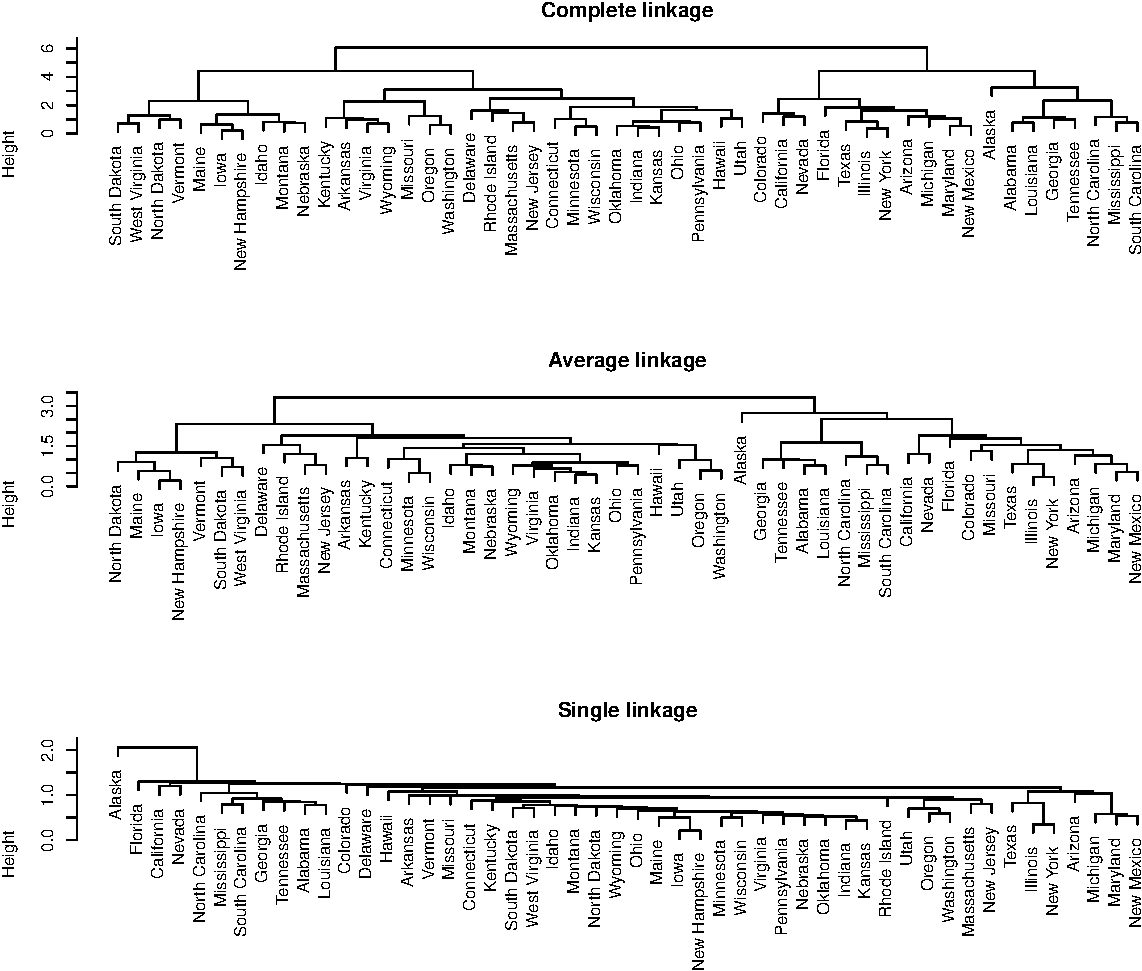
\includegraphics{ch12_lab_files/figure-latex/hclust-usarrests-plots-1} \end{center}

\begin{Shaded}
\begin{Highlighting}[]
\FunctionTok{par}\NormalTok{(}\AttributeTok{mfrow =} \FunctionTok{c}\NormalTok{(}\DecValTok{1}\NormalTok{, }\DecValTok{1}\NormalTok{))}
\end{Highlighting}
\end{Shaded}

The same observations can appear in visibly different positions in the
three dendrograms because the linkage rule changes which merge is
considered closest. A dendrogram is not a final partition until we
choose a height or a number of clusters at which to cut it.

\subsection{Cutting the dendrogram}\label{cutting-the-dendrogram}

\begin{Shaded}
\begin{Highlighting}[]
\NormalTok{complete\_k4 }\OtherTok{\textless{}{-}} \FunctionTok{cutree}\NormalTok{(hc.complete, }\AttributeTok{k =} \DecValTok{4}\NormalTok{)}
\NormalTok{average\_k4 }\OtherTok{\textless{}{-}} \FunctionTok{cutree}\NormalTok{(hc.average, }\AttributeTok{k =} \DecValTok{4}\NormalTok{)}

\FunctionTok{head}\NormalTok{(complete\_k4)}
\end{Highlighting}
\end{Shaded}

\begin{verbatim}
##    Alabama     Alaska    Arizona   Arkansas California   Colorado 
##          1          1          2          3          2          2
\end{verbatim}

\begin{Shaded}
\begin{Highlighting}[]
\FunctionTok{table}\NormalTok{(complete\_k4)}
\end{Highlighting}
\end{Shaded}

\begin{verbatim}
## complete_k4
##  1  2  3  4 
##  8 11 21 10
\end{verbatim}

\begin{Shaded}
\begin{Highlighting}[]
\FunctionTok{table}\NormalTok{(average\_k4)}
\end{Highlighting}
\end{Shaded}

\begin{verbatim}
## average_k4
##  1  2  3  4 
##  7  1 12 30
\end{verbatim}

\begin{Shaded}
\begin{Highlighting}[]
\NormalTok{comparison }\OtherTok{\textless{}{-}} \FunctionTok{table}\NormalTok{(}
  \AttributeTok{Complete\_linkage =}\NormalTok{ complete\_k4,}
  \AttributeTok{Average\_linkage =}\NormalTok{ average\_k4}
\NormalTok{)}
\NormalTok{comparison}
\end{Highlighting}
\end{Shaded}

\begin{verbatim}
##                 Average_linkage
## Complete_linkage  1  2  3  4
##                1  7  1  0  0
##                2  0  0 11  0
##                3  0  0  1 20
##                4  0  0  0 10
\end{verbatim}

The cross-tabulation is a descriptive comparison, not a claim that one
clustering is correct. If two methods place the same states together,
that agreement suggests a stable grouping. Disagreement identifies
observations whose group membership depends on the linkage choice.

\subsection{A reproducible cluster
interpretation}\label{a-reproducible-cluster-interpretation}

\begin{Shaded}
\begin{Highlighting}[]
\NormalTok{complete\_profiles }\OtherTok{\textless{}{-}} \FunctionTok{aggregate}\NormalTok{(}
\NormalTok{  USArrests,}
  \AttributeTok{by =} \FunctionTok{list}\NormalTok{(}\AttributeTok{Cluster =}\NormalTok{ complete\_k4),}
  \AttributeTok{FUN =}\NormalTok{ mean}
\NormalTok{)}
\NormalTok{complete\_profiles}
\end{Highlighting}
\end{Shaded}

\begin{verbatim}
##   Cluster    Murder  Assault UrbanPop     Rape
## 1       1 14.087500 252.7500 53.50000 24.53750
## 2       2 11.054545 264.0909 79.09091 32.61818
## 3       3  5.871429 134.4762 70.76190 18.58095
## 4       4  3.180000  78.7000 49.30000 11.63000
\end{verbatim}

Cluster profiles translate an abstract dendrogram into the original
units. A cluster with a high mean for \texttt{Murder} and
\texttt{Assault}, for example, represents states with higher average
values on those measures in this dataset. It is important to describe
these as profiles rather than causal explanations.

\section{\texorpdfstring{\(K\)-Means
Clustering}{K-Means Clustering}}\label{k-means-clustering}

\subsection{The objective}\label{the-objective}

\(K\)-means requires us to choose the number of clusters \(K\) in
advance. It then assigns each observation to one cluster and chooses
cluster centres to minimise within-cluster sum of squares:

\[
\operatorname{WSS}(C_1,\ldots,C_K)
= \sum_{k=1}^{K}\sum_{i\in C_k}
\|x_i-\bar x_k\|^2.
\]

The algorithm alternates between two steps:

\begin{enumerate}
\def\labelenumi{\arabic{enumi}.}
\tightlist
\item
  assign each observation to its nearest current centre;
\item
  recompute each centre as the mean of the observations assigned to it.
\end{enumerate}

Each step cannot increase the objective, but the procedure can stop at a
local minimum. Consequently, \texttt{nstart} runs the algorithm from
multiple random initialisations and keeps the solution with the smallest
WSS.

\subsection{\texorpdfstring{Applying \(K\)-means to
\texttt{USArrests}}{Applying K-means to USArrests}}\label{applying-k-means-to-usarrests}

\begin{Shaded}
\begin{Highlighting}[]
\FunctionTok{set.seed}\NormalTok{(}\DecValTok{1}\NormalTok{)}
\NormalTok{kmeans\_3 }\OtherTok{\textless{}{-}} \FunctionTok{kmeans}\NormalTok{(USArrests\_scaled, }\AttributeTok{centers =} \DecValTok{3}\NormalTok{, }\AttributeTok{nstart =} \DecValTok{20}\NormalTok{)}
\NormalTok{kmeans\_3}\SpecialCharTok{$}\NormalTok{size}
\end{Highlighting}
\end{Shaded}

\begin{verbatim}
## [1] 13 17 20
\end{verbatim}

\begin{Shaded}
\begin{Highlighting}[]
\NormalTok{kmeans\_3}\SpecialCharTok{$}\NormalTok{centers}
\end{Highlighting}
\end{Shaded}

\begin{verbatim}
##       Murder    Assault   UrbanPop       Rape
## 1 -0.9615407 -1.1066010 -0.9301069 -0.9667633
## 2 -0.4469795 -0.3465138  0.4788049 -0.2571398
## 3  1.0049340  1.0138274  0.1975853  0.8469650
\end{verbatim}

The centres are expressed in standardized units, so a centre of \(1\)
means approximately one standard deviation above the overall feature
mean. The cluster sizes show whether the solution is balanced or
dominated by one large group.

\begin{Shaded}
\begin{Highlighting}[]
\NormalTok{kmeans\_profiles }\OtherTok{\textless{}{-}} \FunctionTok{aggregate}\NormalTok{(}
\NormalTok{  USArrests,}
  \AttributeTok{by =} \FunctionTok{list}\NormalTok{(}\AttributeTok{Cluster =}\NormalTok{ kmeans\_3}\SpecialCharTok{$}\NormalTok{cluster),}
  \AttributeTok{FUN =}\NormalTok{ mean}
\NormalTok{)}
\NormalTok{kmeans\_profiles}
\end{Highlighting}
\end{Shaded}

\begin{verbatim}
##   Cluster    Murder   Assault UrbanPop     Rape
## 1       1  3.600000  78.53846 52.07692 12.17692
## 2       2  5.841176 141.88235 72.47059 18.82353
## 3       3 12.165000 255.25000 68.40000 29.16500
\end{verbatim}

Unlike hierarchical clustering, \(K\)-means does not produce all
possible group sizes in one fitted object. We must fit separate models
for different values of \(K\) if we want to compare them.

\subsection{\texorpdfstring{Choosing \(K\) with an elbow
plot}{Choosing K with an elbow plot}}\label{choosing-k-with-an-elbow-plot}

For each \(K\), the total within-cluster sum of squares measures
compactness. It will always decrease as \(K\) grows, because more
centres give the algorithm more flexibility. We therefore look for an
elbow: a point after which adding another cluster produces only modest
improvement.

\begin{Shaded}
\begin{Highlighting}[]
\FunctionTok{set.seed}\NormalTok{(}\DecValTok{1}\NormalTok{)}
\NormalTok{K\_values }\OtherTok{\textless{}{-}} \DecValTok{1}\SpecialCharTok{:}\DecValTok{8}
\NormalTok{wss\_values }\OtherTok{\textless{}{-}} \FunctionTok{sapply}\NormalTok{(K\_values, }\ControlFlowTok{function}\NormalTok{(K) \{}
  \FunctionTok{kmeans}\NormalTok{(USArrests\_scaled, }\AttributeTok{centers =}\NormalTok{ K, }\AttributeTok{nstart =} \DecValTok{20}\NormalTok{)}\SpecialCharTok{$}\NormalTok{tot.withinss}
\NormalTok{\})}

\FunctionTok{plot}\NormalTok{(K\_values, wss\_values, }\AttributeTok{type =} \StringTok{"b"}\NormalTok{, }\AttributeTok{pch =} \DecValTok{19}\NormalTok{,}
     \AttributeTok{xlab =} \StringTok{"Number of clusters K"}\NormalTok{,}
     \AttributeTok{ylab =} \StringTok{"Total within{-}cluster sum of squares"}\NormalTok{,}
     \AttributeTok{main =} \StringTok{"USArrests: K{-}means elbow plot"}\NormalTok{)}
\end{Highlighting}
\end{Shaded}

\begin{center}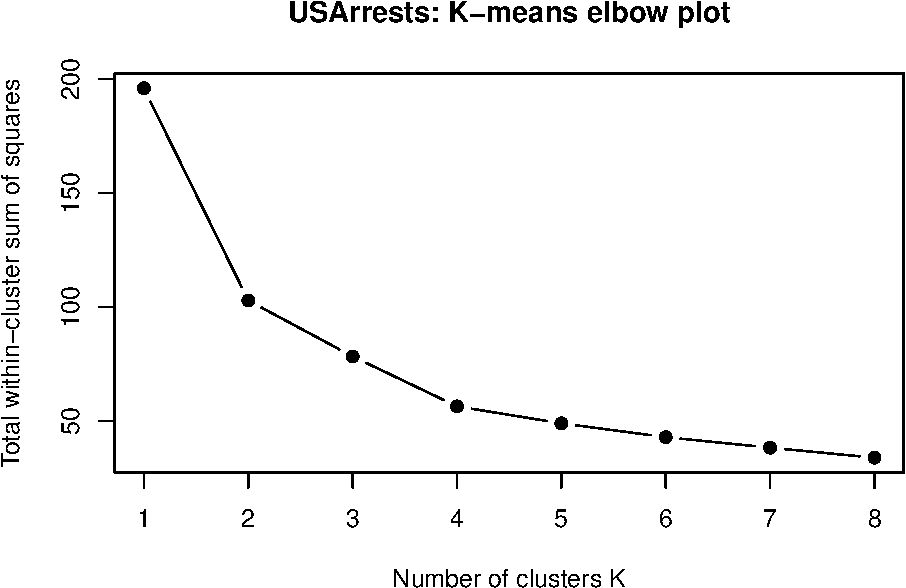
\includegraphics{ch12_lab_files/figure-latex/kmeans-elbow-1} \end{center}

The elbow is a judgement aid rather than a mechanical proof. In an
unsupervised problem there is no response variable that can certify the
best choice, so subject-matter usefulness and stability should also
influence the choice.

\section{\texorpdfstring{The \texttt{NCI60} Gene-Expression
Data}{The NCI60 Gene-Expression Data}}\label{the-nci60-gene-expression-data}

\subsection{Data structure}\label{data-structure}

The \texttt{NCI60} data contain gene-expression measurements for 64
cancer cell lines across thousands of genes. The data object has a
numeric matrix and a label indicating the cancer type. We will use the
labels for interpretation and checking, but unsupervised methods are
fitted using the expression matrix.

\begin{Shaded}
\begin{Highlighting}[]
\FunctionTok{data}\NormalTok{(NCI60)}
\FunctionTok{str}\NormalTok{(NCI60)}
\end{Highlighting}
\end{Shaded}

\begin{verbatim}
## List of 2
##  $ data: num [1:64, 1:6830] 0.3 0.68 0.94 0.28 0.485 ...
##   ..- attr(*, "dimnames")=List of 2
##   .. ..$ : chr [1:64] "V1" "V2" "V3" "V4" ...
##   .. ..$ : chr [1:6830] "1" "2" "3" "4" ...
##  $ labs: chr [1:64] "CNS" "CNS" "CNS" "RENAL" ...
\end{verbatim}

\begin{Shaded}
\begin{Highlighting}[]
\FunctionTok{dim}\NormalTok{(NCI60}\SpecialCharTok{$}\NormalTok{data)}
\end{Highlighting}
\end{Shaded}

\begin{verbatim}
## [1]   64 6830
\end{verbatim}

\begin{Shaded}
\begin{Highlighting}[]
\FunctionTok{table}\NormalTok{(NCI60}\SpecialCharTok{$}\NormalTok{labs)}
\end{Highlighting}
\end{Shaded}

\begin{verbatim}
## 
##      BREAST         CNS       COLON K562A-repro K562B-repro    LEUKEMIA 
##           7           5           7           1           1           6 
## MCF7A-repro MCF7D-repro    MELANOMA       NSCLC     OVARIAN    PROSTATE 
##           1           1           8           9           6           2 
##       RENAL     UNKNOWN 
##           9           1
\end{verbatim}

The raw number of genes is much larger than the number of cell lines.
PCA is therefore a natural first step: it gives a low-dimensional view
of the variation before clustering.

\subsection{\texorpdfstring{PCA for
\texttt{NCI60}}{PCA for NCI60}}\label{pca-for-nci60}

\begin{Shaded}
\begin{Highlighting}[]
\NormalTok{nci60.pca }\OtherTok{\textless{}{-}} \FunctionTok{prcomp}\NormalTok{(NCI60}\SpecialCharTok{$}\NormalTok{data, }\AttributeTok{scale. =} \ConstantTok{TRUE}\NormalTok{)}
\FunctionTok{summary}\NormalTok{(nci60.pca)}
\end{Highlighting}
\end{Shaded}

\begin{verbatim}
## Importance of components:
##                            PC1      PC2      PC3      PC4      PC5      PC6
## Standard deviation     27.8535 21.48136 19.82046 17.03256 15.97181 15.72108
## Proportion of Variance  0.1136  0.06756  0.05752  0.04248  0.03735  0.03619
## Cumulative Proportion   0.1136  0.18115  0.23867  0.28115  0.31850  0.35468
##                             PC7      PC8      PC9     PC10     PC11     PC12
## Standard deviation     14.47145 13.54427 13.14400 12.73860 12.68672 12.15769
## Proportion of Variance  0.03066  0.02686  0.02529  0.02376  0.02357  0.02164
## Cumulative Proportion   0.38534  0.41220  0.43750  0.46126  0.48482  0.50646
##                            PC13     PC14     PC15     PC16     PC17     PC18
## Standard deviation     11.83019 11.62554 11.43779 11.00051 10.65666 10.48880
## Proportion of Variance  0.02049  0.01979  0.01915  0.01772  0.01663  0.01611
## Cumulative Proportion   0.52695  0.54674  0.56590  0.58361  0.60024  0.61635
##                            PC19    PC20     PC21    PC22    PC23    PC24
## Standard deviation     10.43518 10.3219 10.14608 10.0544 9.90265 9.64766
## Proportion of Variance  0.01594  0.0156  0.01507  0.0148 0.01436 0.01363
## Cumulative Proportion   0.63229  0.6479  0.66296  0.6778 0.69212 0.70575
##                           PC25    PC26    PC27   PC28    PC29    PC30    PC31
## Standard deviation     9.50764 9.33253 9.27320 9.0900 8.98117 8.75003 8.59962
## Proportion of Variance 0.01324 0.01275 0.01259 0.0121 0.01181 0.01121 0.01083
## Cumulative Proportion  0.71899 0.73174 0.74433 0.7564 0.76824 0.77945 0.79027
##                           PC32    PC33    PC34    PC35    PC36    PC37    PC38
## Standard deviation     8.44738 8.37305 8.21579 8.15731 7.97465 7.90446 7.82127
## Proportion of Variance 0.01045 0.01026 0.00988 0.00974 0.00931 0.00915 0.00896
## Cumulative Proportion  0.80072 0.81099 0.82087 0.83061 0.83992 0.84907 0.85803
##                           PC39    PC40    PC41   PC42    PC43   PC44    PC45
## Standard deviation     7.72156 7.58603 7.45619 7.3444 7.10449 7.0131 6.95839
## Proportion of Variance 0.00873 0.00843 0.00814 0.0079 0.00739 0.0072 0.00709
## Cumulative Proportion  0.86676 0.87518 0.88332 0.8912 0.89861 0.9058 0.91290
##                          PC46    PC47    PC48    PC49    PC50    PC51    PC52
## Standard deviation     6.8663 6.80744 6.64763 6.61607 6.40793 6.21984 6.20326
## Proportion of Variance 0.0069 0.00678 0.00647 0.00641 0.00601 0.00566 0.00563
## Cumulative Proportion  0.9198 0.92659 0.93306 0.93947 0.94548 0.95114 0.95678
##                           PC53    PC54    PC55    PC56    PC57   PC58    PC59
## Standard deviation     6.06706 5.91805 5.91233 5.73539 5.47261 5.2921 5.02117
## Proportion of Variance 0.00539 0.00513 0.00512 0.00482 0.00438 0.0041 0.00369
## Cumulative Proportion  0.96216 0.96729 0.97241 0.97723 0.98161 0.9857 0.98940
##                           PC60    PC61    PC62    PC63      PC64
## Standard deviation     4.68398 4.17567 4.08212 4.04124 1.237e-14
## Proportion of Variance 0.00321 0.00255 0.00244 0.00239 0.000e+00
## Cumulative Proportion  0.99262 0.99517 0.99761 1.00000 1.000e+00
\end{verbatim}

\begin{Shaded}
\begin{Highlighting}[]
\NormalTok{nci60\_scores }\OtherTok{\textless{}{-}}\NormalTok{ nci60.pca}\SpecialCharTok{$}\NormalTok{x[, }\DecValTok{1}\SpecialCharTok{:}\DecValTok{2}\NormalTok{]}
\NormalTok{nci60\_labels }\OtherTok{\textless{}{-}} \FunctionTok{sort}\NormalTok{(}\FunctionTok{unique}\NormalTok{(}\FunctionTok{as.character}\NormalTok{(NCI60}\SpecialCharTok{$}\NormalTok{labs)))}
\NormalTok{nci60\_label\_codes }\OtherTok{\textless{}{-}} \FunctionTok{match}\NormalTok{(}\FunctionTok{as.character}\NormalTok{(NCI60}\SpecialCharTok{$}\NormalTok{labs), nci60\_labels)}
\FunctionTok{plot}\NormalTok{(nci60\_scores,}
  \AttributeTok{col =}\NormalTok{ nci60\_label\_codes, }\AttributeTok{pch =} \DecValTok{19}\NormalTok{,}
     \AttributeTok{xlab =} \StringTok{"First principal component"}\NormalTok{,}
     \AttributeTok{ylab =} \StringTok{"Second principal component"}\NormalTok{,}
     \AttributeTok{main =} \StringTok{"NCI60 cell lines in the first two PCs"}\NormalTok{)}
\FunctionTok{legend}\NormalTok{(}\StringTok{"topright"}\NormalTok{, }\AttributeTok{legend =}\NormalTok{ nci60\_labels,}
    \AttributeTok{col =} \FunctionTok{seq\_along}\NormalTok{(nci60\_labels), }\AttributeTok{pch =} \DecValTok{19}\NormalTok{,}
       \AttributeTok{cex =} \FloatTok{0.65}\NormalTok{, }\AttributeTok{bty =} \StringTok{"n"}\NormalTok{)}
\end{Highlighting}
\end{Shaded}

\begin{center}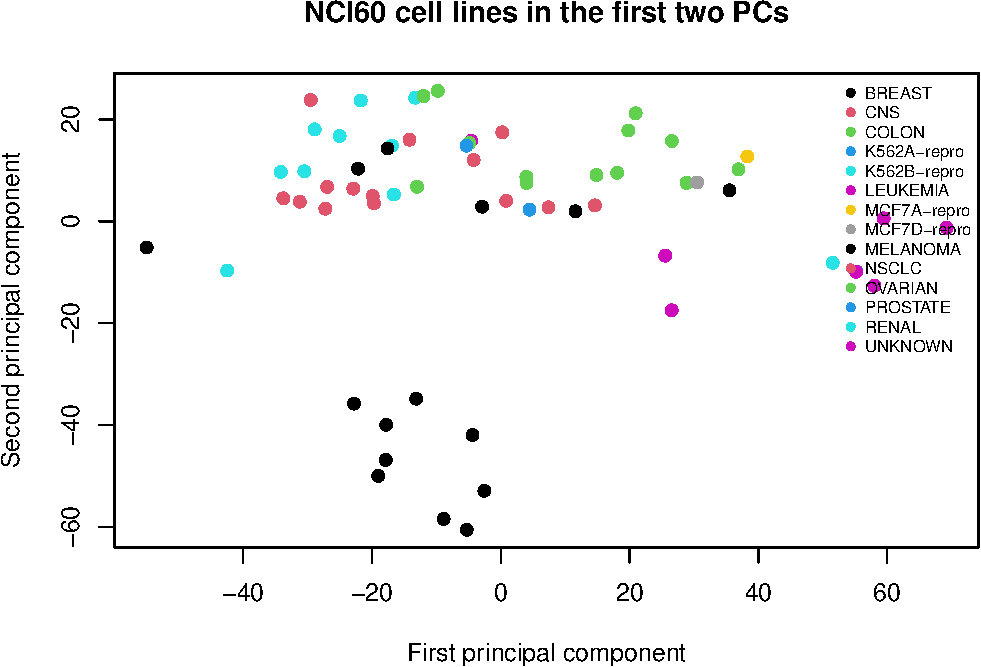
\includegraphics{ch12_lab_files/figure-latex/nci60-pca-plot-1} \end{center}

The colours are added after the unsupervised computation to see whether
known cancer labels line up with visible structure. Strong overlap would
mean that the first two PCs do not separate those types cleanly; visible
grouping would suggest that the expression measurements contain
type-related structure.

\subsection{\texorpdfstring{Hierarchical clustering for
\texttt{NCI60}}{Hierarchical clustering for NCI60}}\label{hierarchical-clustering-for-nci60}

\begin{Shaded}
\begin{Highlighting}[]
\NormalTok{nci60\_distance }\OtherTok{\textless{}{-}} \FunctionTok{dist}\NormalTok{(NCI60}\SpecialCharTok{$}\NormalTok{data)}
\NormalTok{nci60\_hc }\OtherTok{\textless{}{-}} \FunctionTok{hclust}\NormalTok{(nci60\_distance, }\AttributeTok{method =} \StringTok{"complete"}\NormalTok{)}

\FunctionTok{plot}\NormalTok{(nci60\_hc, }\AttributeTok{labels =}\NormalTok{ NCI60}\SpecialCharTok{$}\NormalTok{labs,}
     \AttributeTok{main =} \StringTok{"NCI60: complete{-}linkage clustering"}\NormalTok{,}
     \AttributeTok{xlab =} \StringTok{"Cell lines"}\NormalTok{, }\AttributeTok{sub =} \StringTok{""}\NormalTok{)}
\end{Highlighting}
\end{Shaded}

\begin{center}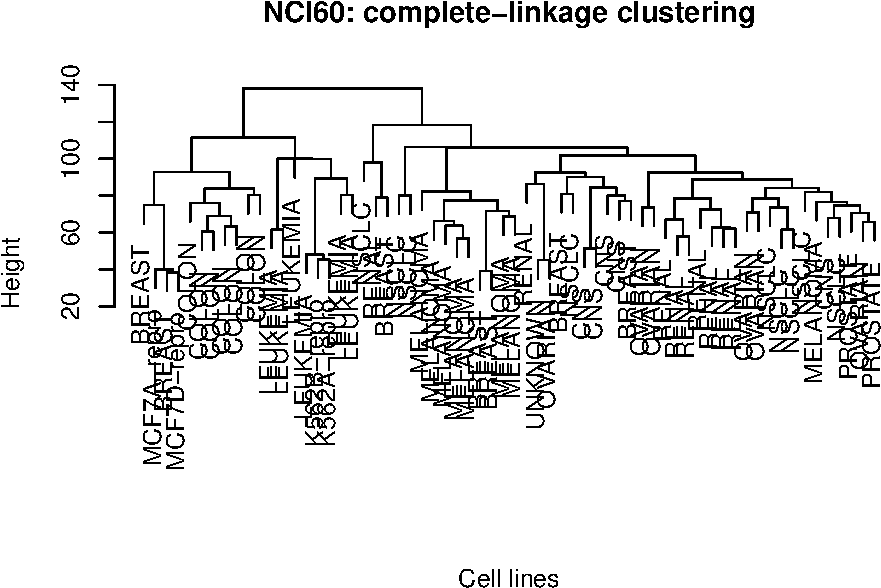
\includegraphics{ch12_lab_files/figure-latex/nci60-hclust-1} \end{center}

\begin{Shaded}
\begin{Highlighting}[]
\NormalTok{nci60\_clusters }\OtherTok{\textless{}{-}} \FunctionTok{cutree}\NormalTok{(nci60\_hc, }\AttributeTok{k =} \DecValTok{4}\NormalTok{)}
\FunctionTok{table}\NormalTok{(}\AttributeTok{Cluster =}\NormalTok{ nci60\_clusters, }\AttributeTok{Cancer\_type =}\NormalTok{ NCI60}\SpecialCharTok{$}\NormalTok{labs)}
\end{Highlighting}
\end{Shaded}

\begin{verbatim}
##        Cancer_type
## Cluster BREAST CNS COLON K562A-repro K562B-repro LEUKEMIA MCF7A-repro
##       1      4   5     0           0           0        0           0
##       2      1   0     0           0           0        0           0
##       3      0   0     0           1           1        6           0
##       4      2   0     7           0           0        0           1
##        Cancer_type
## Cluster MCF7D-repro MELANOMA NSCLC OVARIAN PROSTATE RENAL UNKNOWN
##       1           0        8     8       6        2     8       1
##       2           0        0     1       0        0     1       0
##       3           0        0     0       0        0     0       0
##       4           1        0     0       0        0     0       0
\end{verbatim}

The table compares the unsupervised cluster assignments with the known
labels. It is not a training confusion matrix: the labels were not used
to create the clusters. Some clusters may contain several cancer types,
and one cancer type may appear in multiple clusters, because the
expression structure need not match the supplied labels exactly.

\subsection{\texorpdfstring{\(K\)-means for
\texttt{NCI60}}{K-means for NCI60}}\label{k-means-for-nci60}

\begin{Shaded}
\begin{Highlighting}[]
\FunctionTok{set.seed}\NormalTok{(}\DecValTok{1}\NormalTok{)}
\NormalTok{nci60\_kmeans }\OtherTok{\textless{}{-}} \FunctionTok{kmeans}\NormalTok{(NCI60}\SpecialCharTok{$}\NormalTok{data, }\AttributeTok{centers =} \DecValTok{4}\NormalTok{, }\AttributeTok{nstart =} \DecValTok{50}\NormalTok{)}

\FunctionTok{table}\NormalTok{(}\AttributeTok{Cluster =}\NormalTok{ nci60\_kmeans}\SpecialCharTok{$}\NormalTok{cluster, }\AttributeTok{Cancer\_type =}\NormalTok{ NCI60}\SpecialCharTok{$}\NormalTok{labs)}
\end{Highlighting}
\end{Shaded}

\begin{verbatim}
##        Cancer_type
## Cluster BREAST CNS COLON K562A-repro K562B-repro LEUKEMIA MCF7A-repro
##       1      2   0     0           0           0        0           0
##       2      3   5     0           0           0        0           0
##       3      2   0     7           0           0        0           1
##       4      0   0     0           1           1        6           0
##        Cancer_type
## Cluster MCF7D-repro MELANOMA NSCLC OVARIAN PROSTATE RENAL UNKNOWN
##       1           0        7     0       0        0     0       0
##       2           0        1     6       4        1     9       1
##       3           1        0     3       2        1     0       0
##       4           0        0     0       0        0     0       0
\end{verbatim}

The choice of \(K=4\) is made here for comparison with the hierarchical
cut. In practice, we would examine several values of \(K\), use
stability or validation criteria, and consider the scientific purpose of
the grouping.

\section{Comparing the Methods}\label{comparing-the-methods}

The methods can be summarised by the question each one answers:

{\def\LTcaptype{none} % do not increment counter
\begin{longtable}[]{@{}
  >{\raggedright\arraybackslash}p{(\linewidth - 4\tabcolsep) * \real{0.3333}}
  >{\raggedright\arraybackslash}p{(\linewidth - 4\tabcolsep) * \real{0.3333}}
  >{\raggedright\arraybackslash}p{(\linewidth - 4\tabcolsep) * \real{0.3333}}@{}}
\toprule\noalign{}
\begin{minipage}[b]{\linewidth}\raggedright
Method
\end{minipage} & \begin{minipage}[b]{\linewidth}\raggedright
Main question
\end{minipage} & \begin{minipage}[b]{\linewidth}\raggedright
Main tuning choice
\end{minipage} \\
\midrule\noalign{}
\endhead
\bottomrule\noalign{}
\endlastfoot
PCA & Which directions explain the most variation? & Number of
components \\
Hierarchical clustering & How do observations merge at every distance
level? & Distance, linkage, and cut \\
\(K\)-means & Which \(K\) compact groups minimise within-cluster
variation? & \(K\) and initialisation \\
\end{longtable}
}

A responsible analysis reports the choices that produced the result.
Scaling, distance, linkage, random seed, and the number of clusters are
not cosmetic details; they define the geometry of the unsupervised
problem.

\section{Conclusion}\label{conclusion}

PCA compresses correlated variables into orthogonal directions ordered
by explained variance. Hierarchical clustering provides a nested picture
of similarity, while \(K\)-means produces a direct partition for a
selected \(K\). The \texttt{USArrests} example shows how scaling and
linkage affect a clustering result, and the \texttt{NCI60} example shows
how PCA and clustering can reveal structure in high-dimensional
gene-expression data.

Because unsupervised learning has no response variable to score
directly, the best practice is to examine several reasonable
specifications, report the sensitivity of the conclusions, and interpret
the resulting patterns using subject-matter knowledge rather than
treating one algorithmic output as an objective truth.

\end{document}
